
\subsection{The Partition Coefficient}

This analysis investigated the peak dose rate contribution from various 
radionuclides to the partition coefficient of those radionuclides. 

The partition or distribution coefficient, $K_d$, relates the amount of contaminant adsorbed into the 
solid phase of the host medium to the amount of contaminant adsorbed into the 
aqueous phase of the host medium. It is a common empirical coefficient used to 
capture the effects of a number of retardation mechanisms. The coefficient 
$K_d$, in units of $[m^3\cdot kg^{-1}]$, is the ratio of the mass of contaminant in the 
solid to the mass of contaminant in the solution.

The retardation factor, $R_f$, which is the ratio between velocity of water through a 
volume and the velocity of a contaminant through that volume, can be expressed 
in terms of the partition coefficient,

\begin{align}
  R_f &= 1+\frac{\rho_b}{n_e}K_d
  \label{retardation}
  \intertext{where}
  \rho_b &= ~~\mbox{bulk density}[kg\cdot m^{-3}]\nonumber
  \intertext{and}
  n_e &= ~~\mbox{effective porosity of the medium}[\%].\nonumber
\end{align}




\subsubsection{Parametric Range}

The parameters in this model were all set to the default values except a multiplier 
applied to the partitioning $K_d$ coefficients.

The multiplier took the forty values $1\times10^{-9}, 5\times10^{-8}, \cdots 
5\times10^{10}$ Only the far field partition coefficients were altered by this 
factor. Partition coefficients effecting the EDZ and fast pathway were not 
changed.


\subsubsection{Results}

The expected inverse relationship between the retardation 
factor and resulting peak annual dose was found for all elements that were not 
assumed to be effectively infinitely soluble. In the low retardation coefficient 
cases, a regime is established in which the peak annual dose is entirely 
unaffected by changes in retardation coefficient. For large values of 
retardation coefficient, the sensitivity to small changes in the retardation 
coefficient increases dramatically. In that sensitive regime, the change in peak 
annual dose is inversely related to the retardation coefficient. Between these 
two regimes was a transition regime, in which the $K_d$ factor ranges from $1\times10^{-5}$ to 
$5\times10^{0} [-]$.

It is clear from Figures \ref{fig:KdSumFactor} and \ref{fig:KdSum} that 
for retardation coefficients greater than a threshold, the 
relationship between peak annual dose and retardation coefficient is a strong 
inverse one. 

\begin{figure}[ht]
\centering
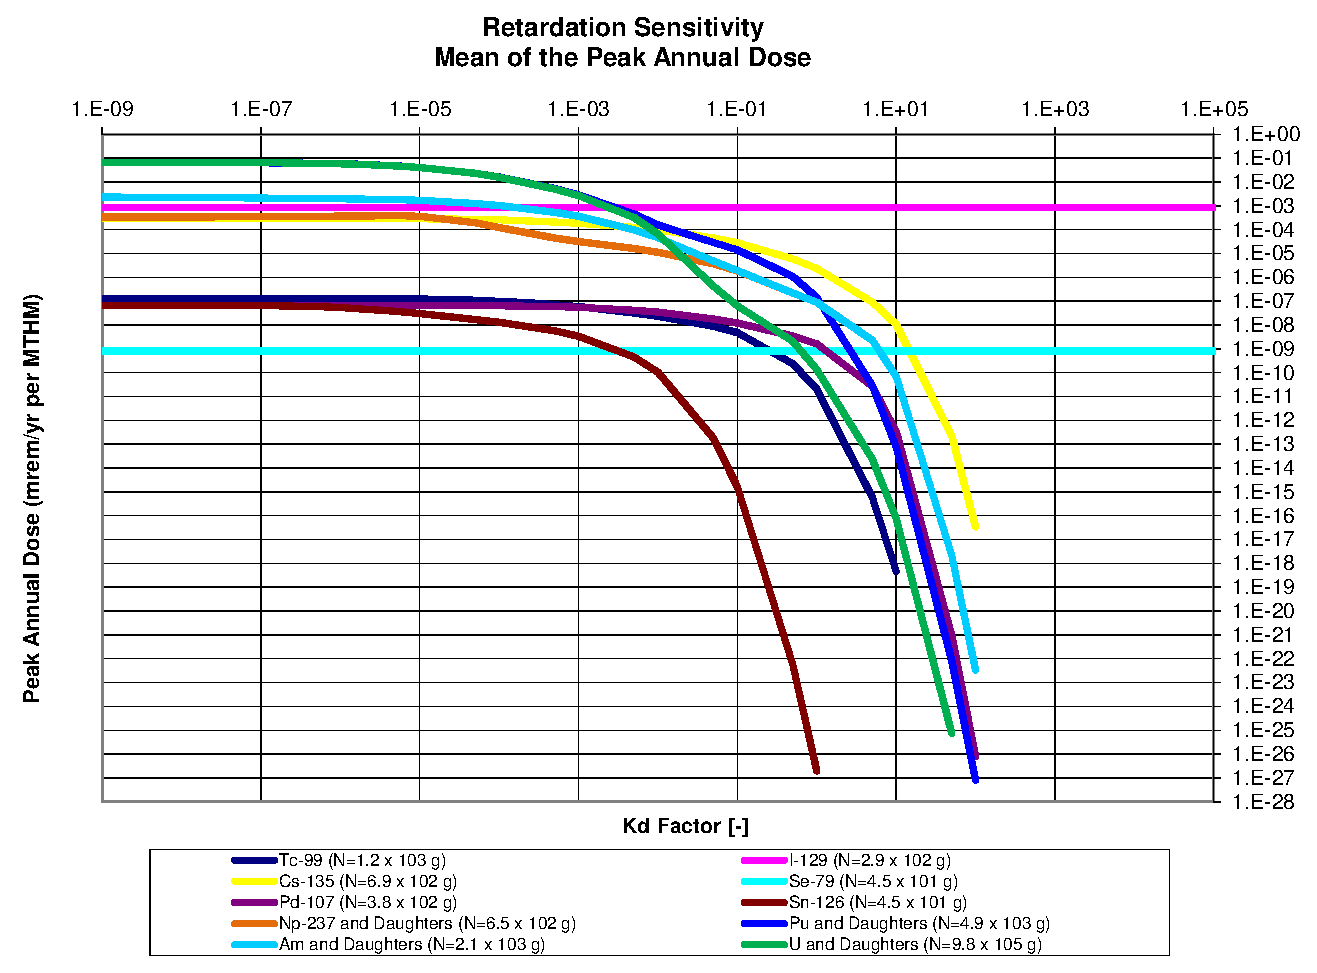
\includegraphics[width=\linewidth]{./chapters/nuclide_sensitivity/clay/Sorption/Retardation_Summary_kdFactor.eps}
\caption{$K_d$ factor sensitivity.  The peak annual dose due to an inventory, 
$N$, of each isotope.}
\label{fig:KdSumFactor}
\end{figure}

\begin{figure}[ht]
\centering
\includegraphics[width=\linewidth]{./chapters/nuclide_sensitivity/clay/Sorption/Retardation_Summary_kd.eps}
\caption{$K_d$ sensitivity.  The peak annual dose due to an inventory, 
$N$, of each isotope.}
\label{fig:KdSum}
\end{figure}

\clearpage
